\begin{frame}
  \frametitle{Adjoints are key ingredients for sensitivity analysis,
    PDE-constrained optimization, ...}

  \vspace{1em}
  So far we have focused on solving forward PDEs.

  \bigskip

  But we want to do (and can do) more than that!

  \bigskip

  Maybe we are interested in ...
  \begin{itemize}
  \item
    the sensitivity with respect to certain parameters
    \begin{itemize}
    \item initial conditions,
    \item forcing terms,
    \item unknown coefficients.
    \end{itemize}
  \item
    PDE-constrained optimization
    \begin{itemize}
    \item
      data assimilation
    \item
      optimal control
    \end{itemize}
  \item
    goal-oriented error control
  \end{itemize}

  \bigskip

  For this we want to compute \alert{functional derivatives} and
  adjoints provide an efficient way of doing so.

\end{frame}

\small
\begin{frame}[fragile]
  \frametitle{What is the sensitivity of the abnormal wave propagation to the local tissue conductivities?}

  The wave propagation abnormality at a given time $T$:
  \begin{align*}
    J(v, s, u) = \| v (T) - v_{\rm obs} (T)\|^2,  \quad
    \alert{\frac{\partial J}{\partial g_{\rm e|i|l|t}} = \; ?}
  \end{align*}
  \begin{python}
v_d = Function(V, "healthy_obs_200.xml.gz")
J = Functional(inner(v - v_d, v - v_d)*dx*dt[T])
dJdg_s = compute_gradient(J, gs)
  \end{python}
  \begin{figure}
    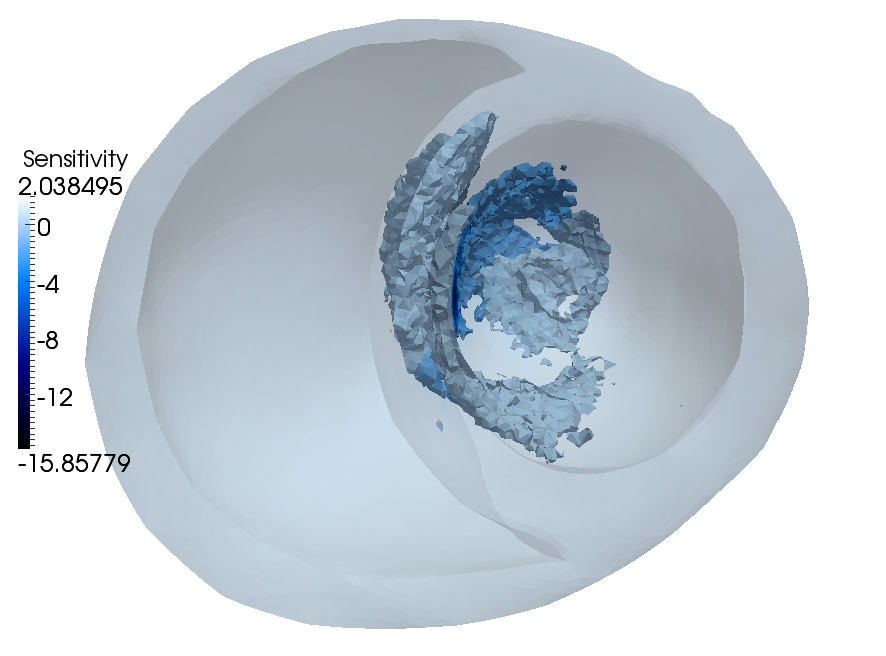
\includegraphics[width=0.24\textwidth]{png/g_el_plusx.png}
    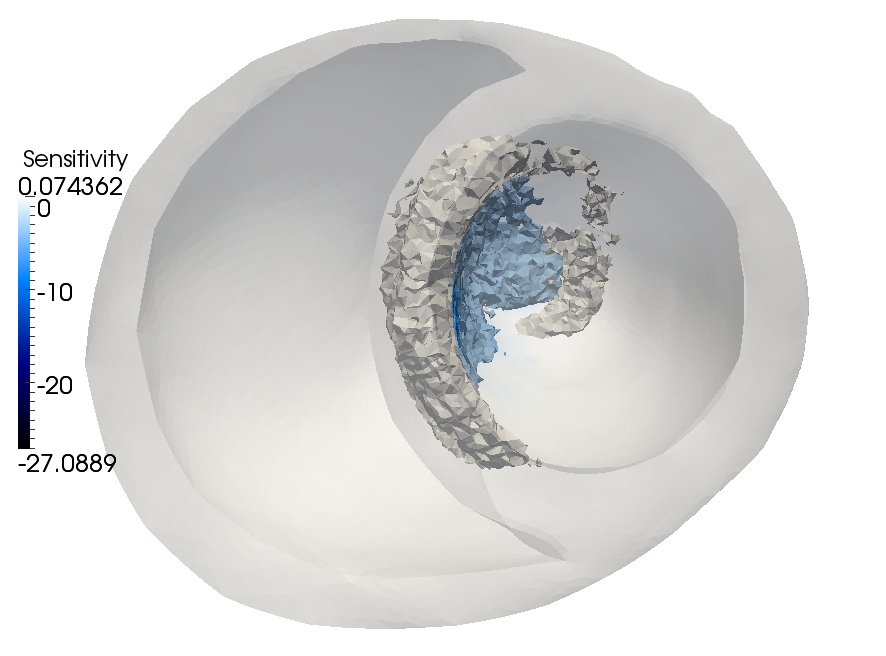
\includegraphics[width=0.24\textwidth]{png/g_et_plusx.png}
    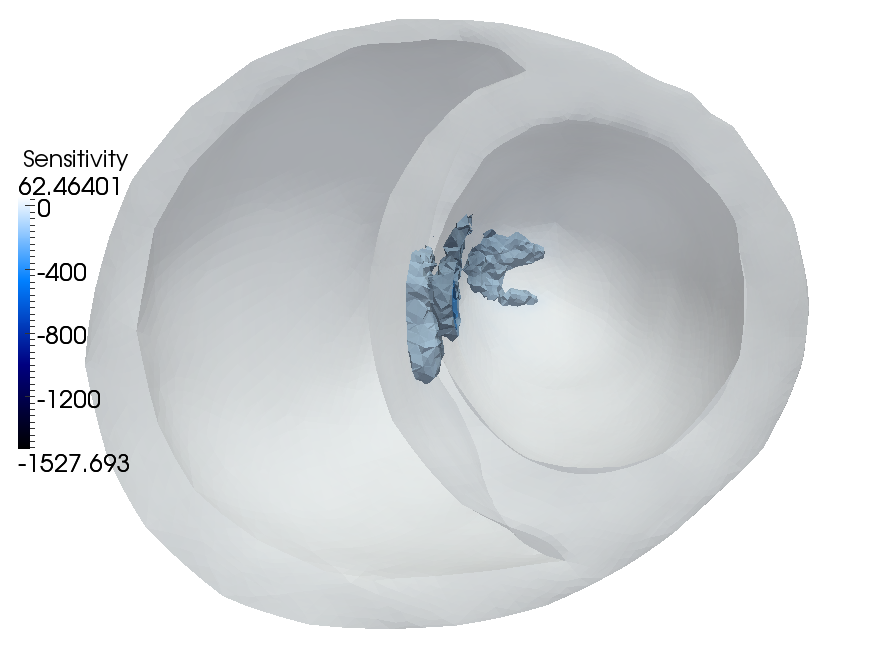
\includegraphics[width=0.24\textwidth]{png/g_il_plusx.png}
    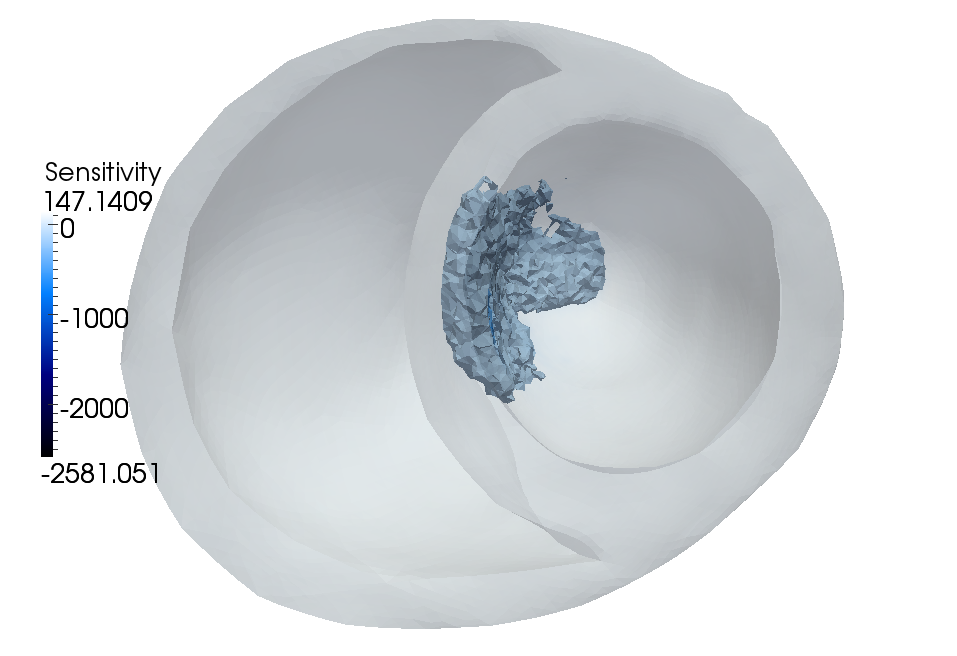
\includegraphics[width=0.25\textwidth]{png/g_it_plusx.png} \\
    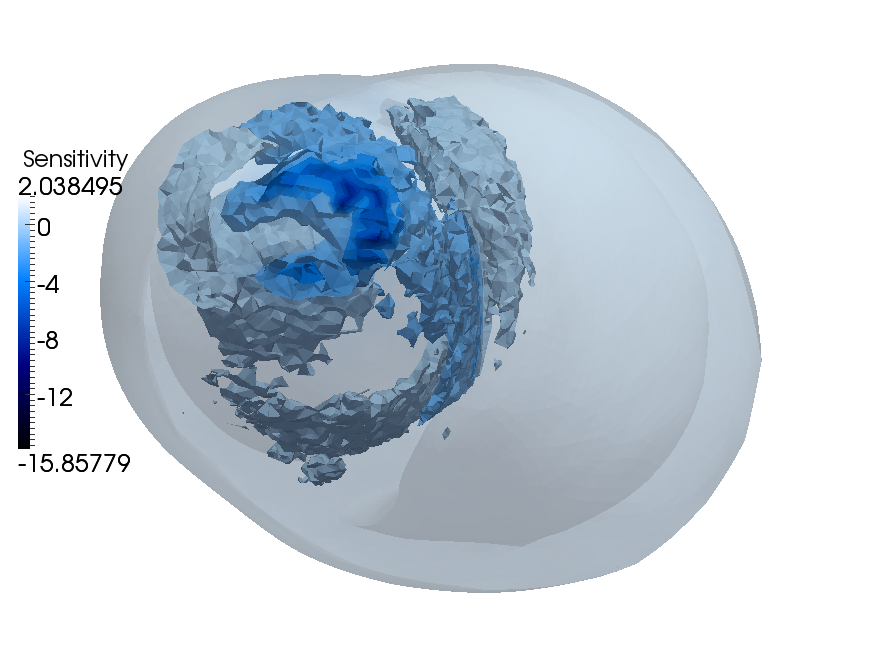
\includegraphics[width=0.24\textwidth]{png/g_el_minusx.png}
    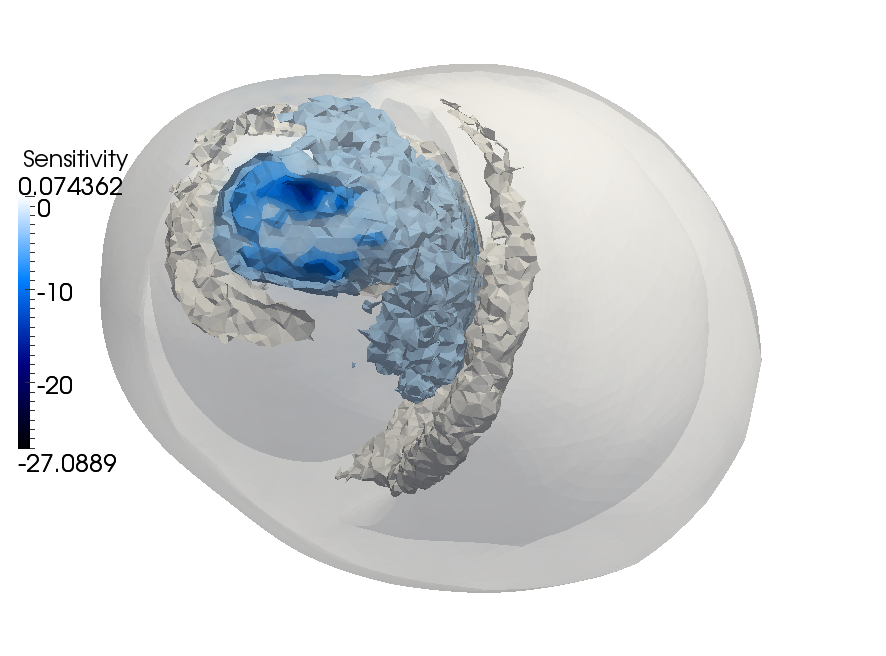
\includegraphics[width=0.24\textwidth]{png/g_et_minusx.png}
    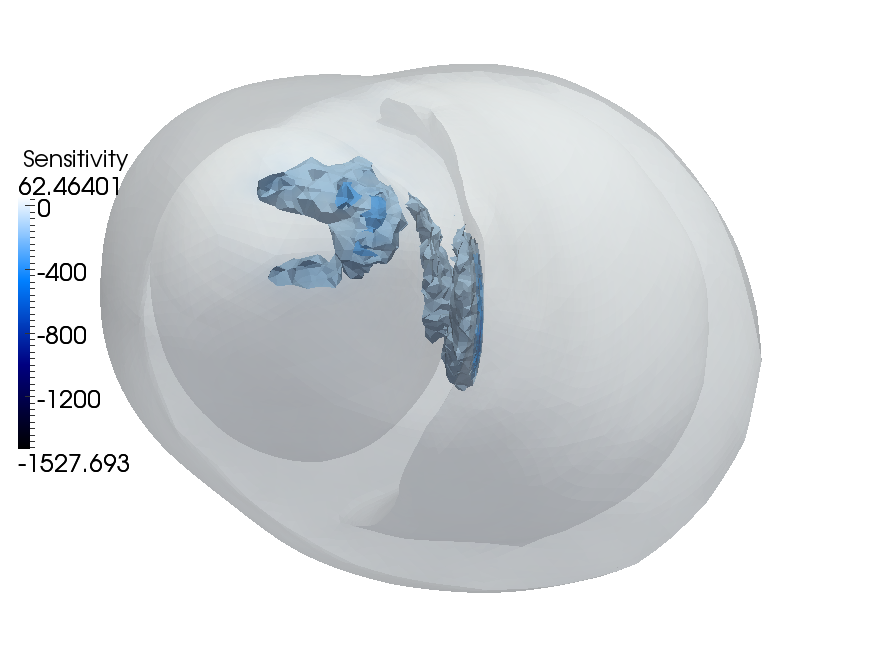
\includegraphics[width=0.24\textwidth]{png/g_il_minusx.png}
    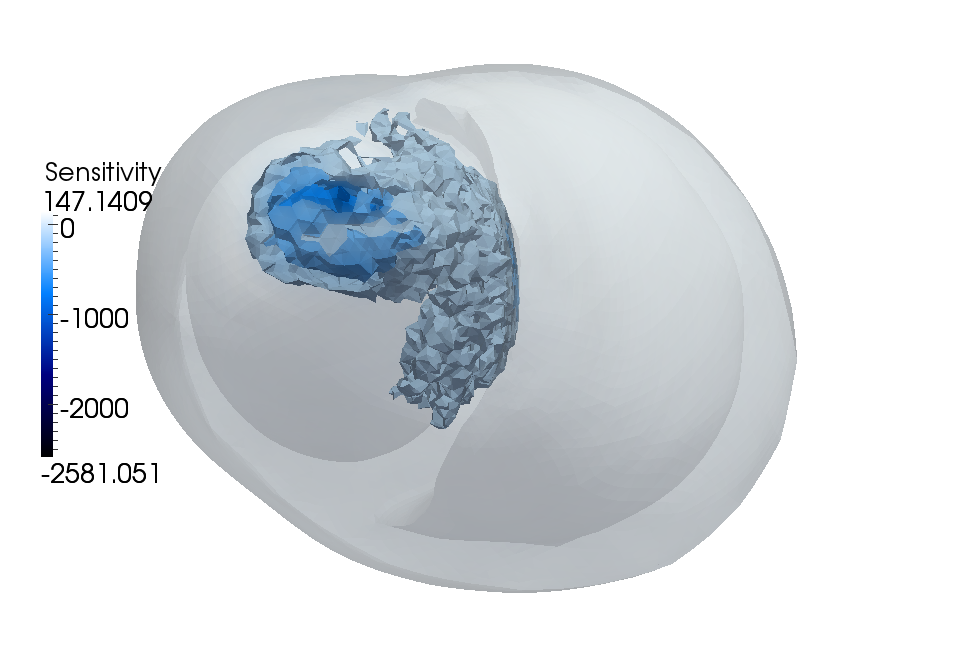
\includegraphics[width=0.25\textwidth]{png/g_it_minusx.png}
  \end{figure}

\end{frame}

\normalsize

\begin{frame}
    \frametitle{The Hello World of functional derivatives}
    Consider the Poisson's equation
    \begin{equation*}
        \begin{aligned}
            - \nu \Delta u = m \quad & \textrm{in } \Omega, \\
            u = 0 \quad & \textrm{on } \partial \Omega,
    \end{aligned}
    \end{equation*}
    together with the \emph{objective functional}
    \begin{equation*}
        J(u) = \frac{1}{2} \int_\Omega \|u - u_d\|^2 \dx,
    \end{equation*}
    where $u_d$ is a known function.

    \begin{block}{Goal}
        Compute the sensitivity of $J$ with respect to the \emph{parameter} $m$: $\textrm{d} J / \textrm{d}m$.
    \end{block}

\end{frame}

\begin{frame}
    \frametitle{Computing functional derivatives (Part 1/3)}
        \begin{block}{Given}
            \begin{itemize}
                \item Parameter $m$,
                \item PDE $F(u, m) = 0$ with solution $u$.
                \item Objective functional $J(u, m) \to \mathbb R$,
            \end{itemize}
        \end{block}

        \onslide<2->{
            \begin{block}{Goal}
                Compute $\textrm{d} J / \textrm{d}m$.
            \end{block}
        }

        \onslide<3->{
        \begin{block}{Reduced functional}
            Consider $u$ as an implicit function of $m$ by solving the PDE.
            With that we define the \emph{reduced functional} $R$:
            \begin{equation*}
                R(m) = J(u(m), m)
            \end{equation*}
        \end{block}
    }

\end{frame}

%\begin{frame}
%    \frametitle{Comput. deriv. (ii) Implicit function theorem}
%        \begin{block}{Implicit function theorem}
%            Let $F$ be continuously Frechet diffentiable and let $\frac{\partial F}{\partial u}$ have a bounded inverse.
%
%            Then:
%            \begin{itemize}
%                \item $F(u, m) = 0$ defines a parameter to state map $u(m)$,
%                \item $u(m)$ is continuously Frechet differentiable. %i.e.
%            %$\frac{\textrm{d} u}{\textrm{d} m} \in C^1$.
%            \end{itemize}
%        \end{block}
%
%\end{frame}

\begin{frame}
    \frametitle{Computing functional derivatives (Part 2/3)}

        Reduced functional:
        \begin{equation*}
            R(m) \equiv J(u(m), m).
        \end{equation*}


        \onslide<2->{
        Taking the derivative of with respect to $m$ yields:
        \begin{equation*}
            \frac{\textrm{d}R}{\textrm{d}m} = \frac{\textrm{d}J}{\textrm{d}m} = \frac{\partial J}{\partial u} \frac{\textrm{d} u}{\textrm{d} m} + \frac{\partial J}{\partial m}.
        \end{equation*}
    }

        \onslide<3>{
Computing $\frac{\partial J}{\partial u}$ and $\frac{\partial J}{\partial m}$ is straight-forward, but how handle $\frac{\textrm{d} u}{\textrm{d} m}$?
    }

\end{frame}

\begin{frame}
    \frametitle{Computing functional derivatives (Part 3/3)}

    Taking the derivative of $F(u, m) = 0$ with respect to $m$ yields:

        \begin{equation*}
            \frac{\textrm{d}F}{\textrm{d}m} = \frac{\partial F}{\partial u} \frac{\textrm{d} u}{\textrm{d} m} + \frac{\partial F}{\partial m} = 0
        \end{equation*}


        \onslide<2->{
        Hence:

        \begin{equation*}
            \frac{\textrm{d} u}{\textrm{d} m} = - \left(\frac{\partial F}{\partial u}\right)^{-1} \frac{\partial F}{\partial m}
        \end{equation*}
    }
        \onslide<3->{

        \begin{block}{Final formula for functional derivative}
            \begin{equation*}
                \frac{\textrm{d}J}{\textrm{d}m} = - \mathrlap{\overbrace{\phantom{\frac{\partial J}{\partial  u} \left(\frac{\partial F}{\partial  u}\right)^{-1} }}^{\textrm{adjoint PDE}}}
                \frac{\partial J}{\partial  u} \underbrace{ \left(\frac{\partial F}{\partial  u}\right)^{-1} \frac{\partial F}{\partial  m}}_{\textrm{tangent linear PDE}} + \frac{\partial J}{\partial  m},
            \end{equation*}
        \end{block}
    }
\end{frame}

\begin{frame}
    \frametitle{Dimensions of a finite dimensional example}

    \vspace{-1em}
    \begin{figure}
    \newlength{\mwidth}
    \newlength{\uwidth}
    \setlength{\mwidth}{1cm}
    \setlength{\uwidth}{2cm}
    \begin{equation*}
        \frac{\textrm{d}J}{\textrm{d}m} =
    \mathrlap{\overbrace{\phantom{
                \fbox{\hspace{0.4\uwidth} $-\frac{\partial J}{\partial  u}$ \hspace{0.4\uwidth}}
                \times
                \fbox{
                \begin{minipage}{\uwidth}
                \vspace{0.5\uwidth}
                \centerline{$\left(\frac{\partial F}{\partial  u}\right)^{-1}$}
                \vspace{0.5\uwidth}
                \end{minipage}
                }
             }}^{\textrm{discretised adjoint PDE}}}
                \fbox{\hspace{0.4\uwidth} $-\frac{\partial J}{\partial  u}$ \hspace{0.4\uwidth}}
            \times
            \underbrace{
                \fbox{
                \begin{minipage}{\uwidth}
                \vspace{0.5\uwidth}
                \centerline{$\left(\frac{\partial F}{\partial  u}\right)^{-1}$}
                \vspace{0.5\uwidth}
                \end{minipage}
                }
                \times
                \fbox{
                \begin{minipage}{\mwidth}
                \vspace{0.5\uwidth}
                \centerline{$\frac{\partial F}{\partial  m}$}
                \vspace{0.5\uwidth}
                \end{minipage}
                }
            }_{\textrm{discretised tangent linear PDE}}
    \hspace{2mm}
    +
    \hspace{2mm}
    \fbox{\hspace{0.25\uwidth} $\frac{\partial J}{\partial  m}$ \hspace{0.25\uwidth}}
    \end{equation*}
    \end{figure}

    The \alert{tangent linear solution} is a matrix of dimension
    $|u|\times |m|$ and requires the solution of $m$ linear systems.

    \bigskip

    The \alert{adjoint solution} is a vector of dimension $|u|$ and
    requires the solution of one linear system.
\end{frame}


%\begin{frame}
%    \frametitle{Tangent linear approach}
%    \begin{enumerate}
%        \item Solve the tangent linear equation
%              \begin{equation*}
%                  \frac{\partial F}{\partial u} \frac{\textrm{d} u}{\textrm{d} m} = - \frac{\partial F}{\partial m}
%              \end{equation*}
%        \item Compute
%        \begin{equation*}
%            \frac{\textrm{d}J}{\textrm{d}m} = \frac{\partial J}{\partial u} \frac{\textrm{d} u}{\textrm{d} m} + \frac{\partial J}{\partial m}
%        \end{equation*}
%
%    \end{enumerate}
%
%    The computational expensive part is (1). Its cost is independent of the number of \emph{output values} but increases with the number of \emph{input variables}.
%\end{frame}
%

\begin{frame}
    \frametitle{Adjoint approach}
    \begin{enumerate}
        \item Solve the adjoint equation for $\lambda$
              \begin{equation*}
                  \frac{\partial F}{\partial u}^*\lambda= - \frac{\partial J^*}{\partial u}.
              \end{equation*}
        \item Compute
        \begin{equation*}
            \frac{\textrm{d}J}{\textrm{d}m} = \lambda^* \frac{\partial F}{\partial m} + \frac{\partial J}{\partial m}.
        \end{equation*}

    \end{enumerate}

    \vspace{1cm}
    The computational expensive part is (1). It requires solving the (linear) adjoint PDE, and its cost is independent of the choice of parameter $m$.
\end{frame}
